\documentclass[11pt,a4paper]{article}
\usepackage[margin=2.5cm]{geometry}
\usepackage[utf8]{inputenc}
\usepackage[T1]{fontenc}
\usepackage{amsmath,amssymb}
\usepackage{graphicx}
\usepackage{booktabs}
\usepackage{hyperref}
\usepackage[round]{natbib}
\usepackage{xcolor}

% Figures produced by the pipeline are read directly from its output folder.
\graphicspath{{figures/}{../pipeline/outputs/figures/}}
\newcommand{\todo}[1]{\textcolor{red}{[TODO: #1]}}

\title{Dengue Surge Warning for Singapore:\\
Predicting Weekly Case Surges from Surveillance and Weather Data}
\author{\todo{Author name}}
\date{\today}

\begin{document}
\maketitle

\begin{abstract}
\todo{Write last. 150--200 words: problem, data, two surge definitions, models compared, main result, implication.}
\end{abstract}

\section{Introduction}
\label{sec:intro}
Dengue is endemic in Singapore and shows recurrent epidemic years. Public-health
action (vector control, communication, hospital capacity) is most effective when it
starts before cases peak, which motivates an early warning of \emph{surges}.

\todo{Motivation, previous work in Singapore \citep{hii2012forecast,shi2016three}.}

\paragraph{Research questions.}
\begin{enumerate}
  \item How should a ``surge'' be defined, and how much do two definitions
        (threshold exceedance vs.\ short-term growth) disagree?
  \item How far ahead (1, 2, 4 weeks) can a surge be predicted from past cases alone?
  \item Do lagged weather variables add predictive value beyond past cases?
  \item Do tree-based models outperform (penalised) logistic regression and count regression?
\end{enumerate}

\section{Data}
\label{sec:data}
\subsection{Dengue cases}
Weekly notified dengue fever and dengue haemorrhagic fever (DHF) cases from the
Ministry of Health weekly infectious disease bulletin (data.gov.sg), 2012--2022.
\todo{number of weeks, missing weeks, note on epidemiological weeks.}

\subsection{Weather}
Daily rainfall, temperature and relative humidity for Singapore from the Open-Meteo
historical archive, aggregated to the same weeks.
\todo{justify source; compare with NEA Changi station if time.}

\begin{figure}[h]
  \centering
  \IfFileExists{../pipeline/outputs/figures/eda_cases_timeseries.png}{
    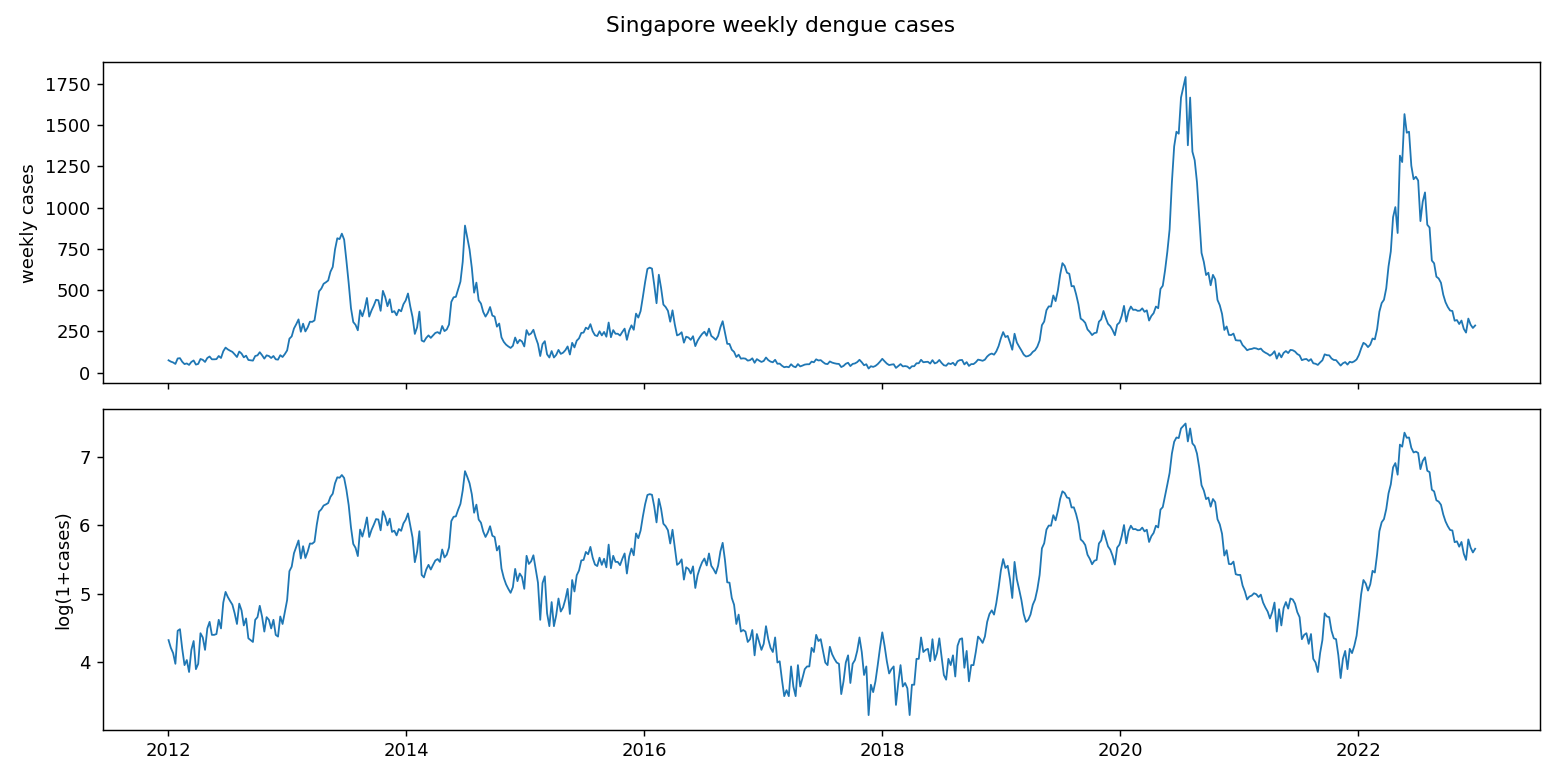
\includegraphics[width=\textwidth]{eda_cases_timeseries.png}}{\fbox{figure pending: run pipeline}}
  \caption{Weekly dengue cases in Singapore.}
  \label{fig:cases}
\end{figure}

\section{Methods}
\label{sec:methods}
\subsection{Surge definitions}
Let $y_t$ be the cases in week $t$ and $h$ the forecast horizon.
\begin{itemize}
  \item \textbf{Threshold (A):} $S^{A}_{t,h} = \mathbb{1}\{y_{t+h} > \mu_t + k\,\sigma_t\}$,
        where $\mu_t,\sigma_t$ are the mean and standard deviation of the previous $W=52$ weeks.
  \item \textbf{Growth (B):} $S^{B}_{t,h} = \mathbb{1}\{y_{t+h} \ge (1+p)\,y_t \;\wedge\; y_{t+h}\ge m\}$.
\end{itemize}

\subsection{Predictors}
All predictors are known at week $t$: lagged log cases, rolling means, recent growth,
seasonal terms $\sin/\cos$ of week-of-year, and weather lagged 0--12 weeks.

\subsection{Models}
Logistic regression (unpenalised and $\ell_1$), a depth-3 classification tree,
random forest, gradient boosting, and Poisson count regressions whose forecasts are
converted to alarms with the same rule that defines the target.

\subsection{Validation and model selection}
Rolling-origin evaluation: each year from 2017 is a test fold, trained on all earlier
weeks, with the last $h$ weeks purged to avoid target leakage. Metrics: ROC-AUC,
PR-AUC (preferred under class imbalance), Brier score, precision, recall and false alarm rate.

\section{Results}
\label{sec:results}
\subsection{Exploratory analysis}
\todo{seasonality, epidemic years, lagged correlations (eda\_summary.md).}

\subsection{Target definitions}
\todo{prevalence and agreement of A vs.\ B (features\_summary.md).}

\subsection{Model comparison}
\todo{table from outputs/tables/model\_cv\_pooled.csv.}

\subsection{Interpretation}
\todo{feature importance, tree rules.}

\section{Discussion}
\label{sec:discussion}
\todo{what works, value of weather, limitations (national level only, reporting changes,
2020 COVID-19 period, data ends 2022), operational use.}

\section{Conclusion}
\label{sec:conclusion}
\todo{}


\bibliographystyle{plainnat}
\bibliography{references}
\end{document}
